\documentclass[a4paper, oneside]{article}
\usepackage[T1]{fontenc}
\usepackage[utf8]{inputenc}
\usepackage[english]{babel}
\usepackage{frontespizio}
\usepackage{graphicx}
\usepackage{listings}
\usepackage{scrextend}
\usepackage[margin=1.2in]{geometry}
\usepackage[font=small,labelfont=bf]{caption}
\usepackage{url}
\usepackage{verbatim}

\begin{document}
\selectlanguage{english}
\baselineskip 13pt

% ---- FRONTESPIZIO ----- 
\begin{frontespizio} 
 \Preambolo{\renewcommand{\frontpretitlefont}{\fontsize{15}{12}\scshape}}
\Istituzione {University of Pisa}
\Divisione {Scuola di Ingegneria}
\Corso [Laurea]{Artificial Intelligence and Data Engineering}
\Annoaccademico {2019--2020}
\Titolo {Task2 documentation}
\Filigrana [height=4cm,before=0.28,after=1]{./images/stemma_unipi.png}
\Rientro {1cm}
\Candidato {Giacomo Mantovani}
\Candidato {Stefano Poleggi}
\Relatore {Prof. Pietro Ducange}
 \Punteggiatura {}
\end{frontespizio}

\clearpage

% ----- INDICE -----
	\tableofcontents\thispagestyle{empty}
	\clearpage


\section{Introduction}\pagenumbering{arabic}
The \textbf{<Name of the app>} application offers a real-time sentiment analysis service. When the application starts, the user can perform a sentiment analysis by searching for a topic in the search bar and the application will start extracting tweets analyze them.
The result is printed into a graph which shows the number of tweet analyzed so far and the semtiment rating. The graph keeps updating until the user clicks the stop button or when the application is closed. Moreover the application provides some charts to check the results obtained.
\vspace{5mm}
\begin{figure}[h]
\centering
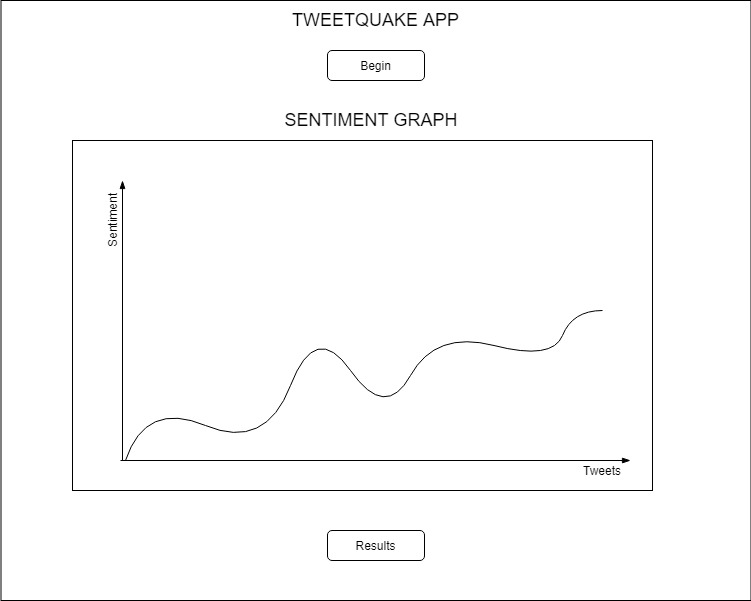
\includegraphics[width=\textwidth]{./images/diagrams/HomeMockup} 
\caption{Home Page Mockup}
\label{fig:mockup}
\end{figure}

\begin{figure}[h]
\centering
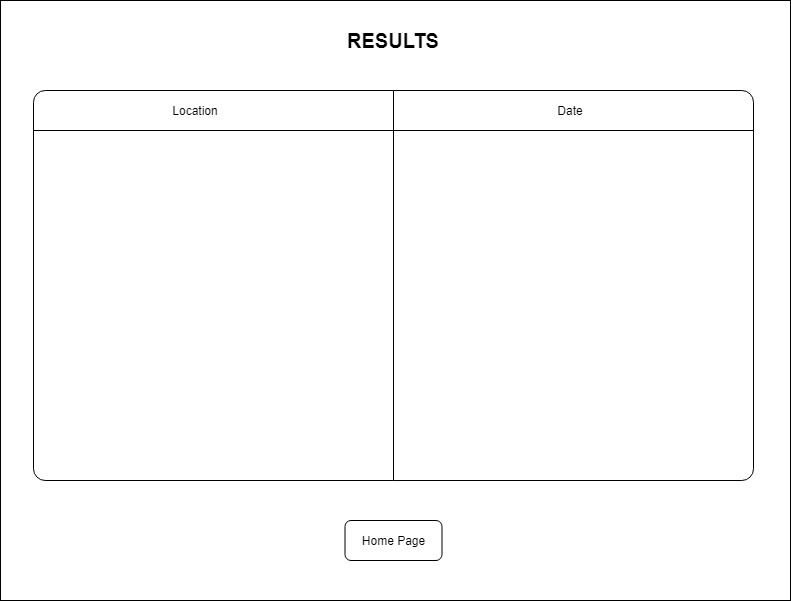
\includegraphics[width=\textwidth]{./images/diagrams/Charts} 
\caption{Results Page Mockup}
\label{fig:mockup}
\end{figure}

\clearpage

\section{Analysis and workflow}

% ----- REQUIREMENTS -----
\subsection{Requirements}

\subsubsection{Functional requirement}
The system has to allow the user to carry out basic functions such as:
\begin{itemize}
\item To select a topic.
\item To retrive the sentiment analysis of the selected topic.
\end{itemize}
The system has to perform the following operations: 
\begin{itemize}
\item Real-time fetching of tweets of a specified topic.
\item Perform a sentiment analysis of the tweets and obtain the sentiment (positive, negative or neutral).
\item When a negative tweet trend is recognized send a notification.
\item perform a visual analysis by filling charts
\end{itemize}
\vspace{2mm}

\subsubsection{Non-functional requirements}
\begin{itemize}
\item Usability, ease of use and intuitiveness of the application by the user.
\item Avaliablility, with the service guaranteed h24.
\item The system should support simultaneous users.
\item The system should provide access to the database with a few seconds of latency.
\end{itemize}

\clearpage

% ----- USE CASES -----
\subsection{Use Cases}

\textbf{Actors}
\begin{itemize}
\item{User: this actor represents a user of the application}
\end{itemize}

\subsubsection{Use Cases Description}
\begin{table}[h]
\centering
\begin{tabular}{p{0.16\textwidth}p{0.2\textwidth}lp{0.5\textwidth}}
\hline
\textbf{Event} & \textbf{UseCase} & \textbf{Actor(s)} & \textbf{Description}\\ \hline
Log in, Log out & Login,  Logout & Admin, User & The user logs in/out the application.\\ \hline
Display all the Films & Browse, Find, Display Films & User, Admin & The user chooses that he wants to view the list of Films. The system browses the data on the db and returns them on the interface.\\ \hline
View Statistics & View Top Rated Films, View Top Productions, View Top Film-maker Countries, View Most Active Users & Admin & The Admin clicks on the button to view the statistics. The system browses on the db the informations used in the calculation and display the result.\\ \hline
Add a film & Add Film & Admin & The admin submits the Film information. The system updates the db and the interface.\\ \hline
Update a film & Update Film & Admin & The admin selects the film and commits the new informations. The system updates the db and the interface.\\ \hline
Delete a film & Delete Film & Admin & The admin selects the film and submits the delete. The system updates the db and the interface.\\ \hline
View the film informations & Select Film, Display Film Info & User, Admin & The user selects the film. The system shows the film informations on the interface.\\ \hline
Vote a film & Vote Film & User, Admin & The user submits the vote on a selected film. The system updates the db and the interface.\\ \hline
\end{tabular}
\end{table}

\begin{minipage}{\linewidth}
\begin{center}
\vspace{8mm}
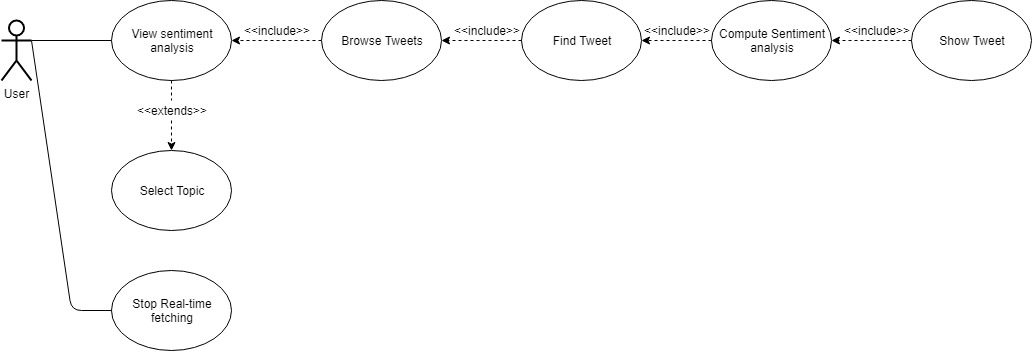
\includegraphics[ width=0.7\textheight]{./images/diagrams/UseCase} 
\captionof{figure}{Use cases diagram}
\vspace{3mm}
\end{center}
\end{minipage}


\clearpage


\subsection{Analysis of entities}
This diagram represents the main entities of the application and the relations between them.
\begin{minipage}{\linewidth}
\begin{center}
\vspace{4mm}
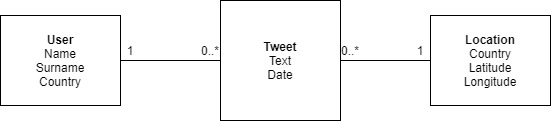
\includegraphics[width = 0.2\textwidth]{./images/diagrams/Uml Analysis diagram} 
\vspace{2mm}
\captionof{figure}{UML analysis diagram}
\label{fig:useCases}
\end{center}
\end{minipage}



\clearpage
% ----- DESIGN -----
\section{Design}

\subsection{Database Choice}
After the analysis phase, which has been carried out so far, we start with the design of the \textbf{<Name of the app>} application. We decide to use MongoDB as data support. Its document-based structure is very useful for the large amount of data that we need to maintain and access, as well as its high scalability, qualities that we do not find in a relational database.
\subsection{Software architecture}
The application is designed over 3 different layers, see figure \ref{fig:architecture_diagram}:
\begin{itemize}
\item Front-end
\item Middleware
\item Back-end
\end{itemize}
\vspace{5mm}
\begin{minipage}{\linewidth}
\begin{center}
\vspace{1mm}
\includegraphics[height = 100mm]{./images/diagrams/architecture} 
\vspace{6mm}
\captionof{figure}{Software architecture diagram\\}
\label{fig:architecture_diagram}
\end{center}
\end{minipage}
\vspace{7mm}
\clearpage

\iffalse

\subsection{Populating the database}
The dataset used in the \textbf{Moviegram} application was created by scraping the Open Movie Database, using their API (\url{http://www.omdbapi.com/}). Given a movie title, this API returns all the information in the OMDb about that movie. Before started building up the dataset using the API, it was necessary to obtain a list of movie titles, to be passed to the API; the list of titles was built up using different web pages as sources:
\begin{itemize}
\item a page of Wikipedia was scraped
\item the pages referring to each year from 2007 to 2021 on the site \url{https://www.wildaboutmovies.com/} were scraped
\item a csv file in the GitHub repository \url{https://github.com/fivethirtyeight/data} was used
\end{itemize}
Once the titles’ list was ready, the only thing left to do was to obtain the key requested by the OMDb API to download the films’ information. Each key provided by the database allows a user to download 1000 film’s information per day. Once the movies’ list and the keys were ready, we could start to use our scraping application.\\

\begin{minipage}{\linewidth}
\begin{center}
\vspace{1mm}
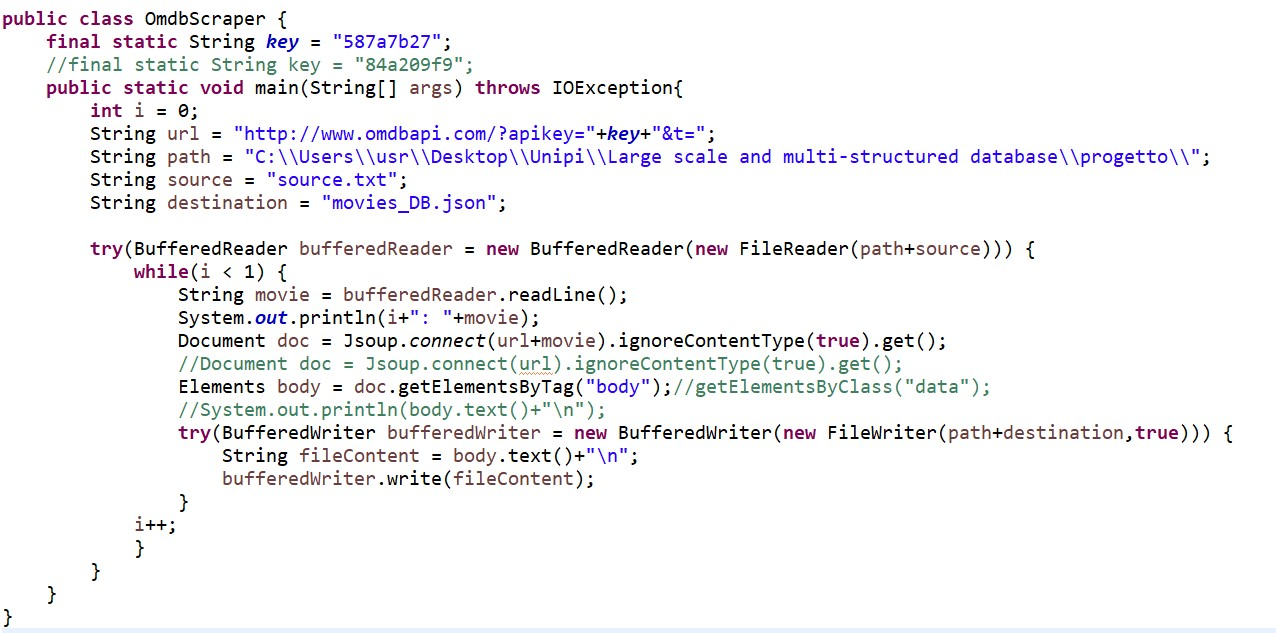
\includegraphics[height = 80mm]{./images/screens/OMDBScraperScreen.jpg} 
\vspace{6mm}
\captionof{figure}{Java class of OMDBScraper\\}
\label{fig:OMDBScraper}
\vspace{4mm}
\end{center}
\end{minipage}
Using our “OmdbScraper” application, we managed to obtain the collection of movies’ information in a JSON format.\\ The format of our JSON elements are the following:\\

\begin{minipage}{\linewidth}
\begin{center}
\vspace{1mm}
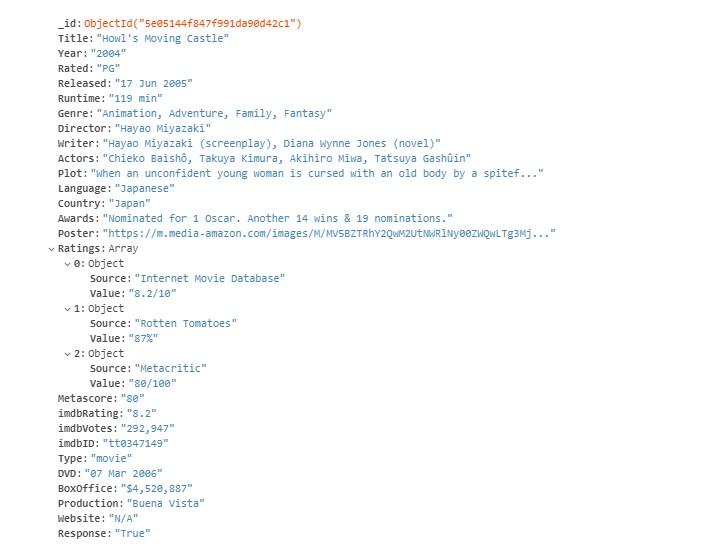
\includegraphics[height = 94mm]{./images/screens/elementJSONExample.jpg} 
\vspace{6mm}
\captionof{figure}{Example of JSON document\\}
\label{fig:elementJSONExample}
\vspace{5mm}
\end{center}
\end{minipage}
We integrated our movies dataset with a plot dataset, found on \url{kaggle.com} (wiki\_plot). In order to do so, we searched for matching between the plot’s movie title and the movie title in our collection; once the matching was found, the plot field in the original element was replaced with the data presents in the plot dataset.\\
Moreover, we managed some data types because, scraping the OpenMovie platform, we'd obtained every field in a string format, but to compute the analytics operations described in the functional requirements section, we need to have some fields in a number format. We ran the following javascript code on the mongo shell, to perform the conversion:
\vspace{2mm}
% ----- android wearable module -----
\begin{lstlisting}[language=Java,  basicstyle=\footnotesize]
	db.collection.find().foerEach( function(x){
		x.ratingImdb = parseFloat( x.imdbRating);
		db.collection.save(x);
	});
\end{lstlisting}
\vspace{5mm}

Finally, for the users' information, we didn't use any kind of scraping or sources. We just created a collection with a few documents, one for each of us, leaving this part of the database as a prototype for future public use. Every user has maintained in the db his name, username, password, and country, as well as a list with the titles of the movies he voted and the relative vote.
% inserire immagine di un documento utente 
\begin{comment}
	{
		Name:"Alice",
		Username:"alice",
		Password:"alice",
		Country:"Italy"
		Numrates:"0",
		Rated:
		[
			{Movie:"", Rate:"", Timestamp:""},
			{Movie:"", Rate:"", Timestamp:""},
			...
		}
	}
\end{comment}
In the film collection, on the other hand, the list of users who voted for each film is not kept, but only a field that keeps the number of votes received (\textit{imdbVotes}) and one that keeps the average vote (\textit{imdbRating}).

% ----- INDEXES -----
\subsection{MongoDb indexes}
\subsubsection{Index 1}
The first index introduced is related to the users collection. This collection is indexed using 'Numrates', a counter for the number of rates that a user has given.
This index will improve the performance of the operation that returns the ranking of the most active users on the plattform.
\begin{verbatim}
     db.users.createIndex({"Numrates" : -1 });
\end{verbatim}
\subsubsection{Index 2}
In order to speeding up the operation that displays the top rated movies related to a specific country, we introduce 2 indexes on the fields 'Country' and 'Ratings'. Theese 2 indexes decrease the performance of the operation that displays the top movies, not considering the country, but we expect the previous operation to be compute more frequently.
\begin{verbatim}
     db.films.createIndex({"Country" : 1, "imdbRating" : -1});
\end{verbatim}

% ----- ANALYTICS -----
\subsection{Analytics and statistics}
\subsubsection{View the top production houses}
This analytic is performed to display all production houses.
\subsubsection{Top rated movies by year and country}



\clearpage

% ----- IMPLEMENTATION -----
\section{Implementation}
\subsection{Used technologies}
The application is developed in java programming language, version 11.0.4, and in JavaFX system to create the GUI, version 11, so it should run on each platform in which JVM is installed, but the application is tested and guardantee on Ubuntu 16 and Window OS. Moreover Maven is used  to build and mantain the project, version 3.8.0. \\
The java driver for mongo manage the comunication between client application layer and mongo backend layer, version 3.11.2.\\ 
For the backend layer it is used MongoDB, version 4.2.\\
So this application is tested using these technologies, considering these particular versions: for other versions the correct execution isn't guaranteed .\\

\subsection{Replica setup}
The following code shows how it is realized the architecture in which 3 mongo server are running in back end layer:
\vspace{2mm}
% ----- android wearable module -----
\begin{lstlisting}[language=Java,  basicstyle=\footnotesize]
# ----- PREPARAZIONE CARTELLE PER LOG E PER I DB -----
sudo mkdir -p /srv/mongodb/rs0-0 /srv/mongodb/rs0-1 /srv/mongodb/rs0-2
sudo mkdir -p /var/log/mongodb/rs0-0 /var/log/mongodb/rs0-1 /var/log/mongodb/rs0-2

# ----- RUN 3 ISTANCES OF MONGOD -----
sudo mongod --port 27017 --dbpath /srv/mongodb/rs0-0 --replSet rs0 --oplogSize 128
--logpath /var/log/mongodb/rs0-0/server.log --fork
sudo mongod --port 27018 --dbpath /srv/mongodb/rs0-1 --replSet rs0 --oplogSize 128 
--logpath /var/log/mongodb/rs0-1/server.log --fork
sudo mongod --port 27019 --dbpath /srv/mongodb/rs0-2 --replSet rs0 --oplogSize 128 
--logpath /var/log/mongodb/rs0-2/server.log --fork

# ----- CHECK LISTENING PROCESS -----
netstat -tulpn

# ----- CONNECT TO PRIMARY MONGOD ISTANCE -----
mongo --port 27017

/* JS SCRIPT */
var rsconf = {
    _id: "rs0",
    members: [
                {_id: 0,  host: "127.0.0.1:27017"},
                {_id: 1,  host: "127.0.0.1:27018"},
                {_id: 2,  host: "127.0.0.1:27019"}
            ]
};
rs.initiate( rsconf );
rs.conf();
rs.status();

# ----- KILL PROCESS USING PORT -----
sudo fuser -k 27017/tcp
sudo fuser -k 27018/tcp
sudo fuser -k 27019/tcp

# ----- ELIMINA CARTELLE ------
sudo rm -r /srv/mongodb/rs0-0 /srv/mongodb/rs0-1 /srv/mongodb/rs0-2
sudo rm -r /var/log/mongodb/rs0-0 /var/log/mongodb/rs0-1 /var/log/mongodb/rs0-2

\end{lstlisting}
\vspace{5mm}
\subsection{Java class description}
\subsubsection{Declaration of class Film}
The following java-code shows a declaration of the class Film.
\vspace{2mm}
\\ <code here>
\vspace{5mm}

\subsubsection{Declaration of class User}
The following java-code shows a declaration of the class User.
\vspace{2mm}
	\\ <code here>
\vspace{5mm}

 Another foundamental class is MongoManager, that manages the db-connection and the related operations.
 The implementation of a set of CRUD operations is desribed as follows.


\subsection{Create}
Adding one or more films to the database using a json document as input.
\vspace{2mm}
 \\<Code here>
\vspace{5mm}

\subsection{Read}
This functionality returns a list of films searched by title. A film is returned if its title contains a piece of the searched title (case insensitive).\\
\vspace{2mm}
\\<code here>
\vspace{5mm}

\subsection{Update}
This operation allows users to update their vote about a selected film.\\
\vspace{2mm}
\\<code here>
\vspace{5mm}

\subsection{Delete}
This operation allows an admin to remove a selected film from the database.\\
\vspace{2mm}
\\<code here>
\vspace{5mm}

\clearpage

\subsection{Analytics}
In this phase the analytics operations that a user is able to perform on the database are shown.

\subsection{GUI}
There are three fxml documents, one for each page of the application, which describes the objects showed in the GUI interface of the related page.
\begin{itemize}
\item Home.fxml
\item Login.fxml
\item Register.fxml
\end{itemize}
In addiction there are 3 classes, called Controllers, that are in charge of handling events of the objects defined in the associated fxml document.
\begin{itemize}
\item HomeController.java
\item LoginController.java
\item RegisterController.java
\end{itemize}

\clearpage
% MANUAL%
\section{User Manual}
When you first run the application, the interface you get is the login one, figure~\ref{fig:screen0}. \\

<login page image--> image name: screen0>\\

In case you are not registered you can click the link at the bottom of the page to be redirected to a register page, figure~\ref{fig:screen1}, otherwise you can sign in the application and by default you get the interface shown in figure~\ref{fig:screen2}\\

<register page image --> image name: screen1>\\

<Application home page after login --> image name: screen2> \\

From here you can search for a film by typing in the relative field and clicking the search button. You'll get a list of films that contains the text entered in the table below. Now you can select a film from the table and all the informations will be shown in the right pane of the application, figure~\ref{fig:screen3}. In the bottom right you are able to add a vote from 1 to 10 for the selected film.\\

<homepage after searching a film and selectiong one --> image name: screen3>\\

In the top left of the page there are two tabs. by default after the login you are in the Home tab, by clicking the Analytics Tab you will see the following page.

<analytics tab page --> image name: screen4>\\

Here you have a choice box (left) to select what kind of analytics you want to be performed from the existing ones, and another one to apply a filter (right), figure~\ref{fig:screen5}. \\

<default analytics page --> image name: screen5>\\

After selecting an analytics you will see the results in the table below, and for some of them you will get a piechart aswell, figure~\ref{fig:screen6}\\

<analytics page after performing analytics -->image name: screen6>\\

To log out, just click on the appropriate button at the bottom.

\clearpage
%ADIMN MANUAL%
\subsection{Admin Manual}
If you have an admin user, you are entitled to make changes on the film lists. You need to log in inserting your username and password, and the application will recognize you as the administrator and show up a third tab called "Admin", figure~\ref{fig:admin0}\\

<page of the admin tab --> image name: admin0>\\

In the Admin tab you can search for a film the same way the user did in the Home tab and after selecting one you are able to delete it by clicking the "Delete" button. On the right pane you are able to insert a json document in the text field, that represent a film in the database, and by clicking the Add button you will insert one or more films in the database (fig.~\ref{fig:admin1}).\\ 

<admin tab after searching films and with a json document in the text field --> image name: admin1>

\fi
\end{document}
